\documentclass[11pt,a4paper]{article}
\usepackage[utf8]{inputenc}
\usepackage[T1]{fontenc}
\usepackage{geometry}
\usepackage{graphicx}
\usepackage{fancyhdr}
\usepackage{tikz}
\usepackage{tabularx}
\usepackage{booktabs}
\usepackage{xcolor}
\usepackage{amsmath}
\usepackage{listings}
\usepackage{hyperref}

% Page setup
\geometry{margin=1in}
\pagestyle{fancy}
\fancyhf{}
\fancyhead[L]{MHT1803 500W Amplifier}
\fancyhead[R]{User Manual v1.0}
\fancyfoot[C]{\thepage}

% TikZ libraries
\usetikzlibrary{shapes,arrows,positioning}

% Colors
\definecolor{primaryblue}{RGB}{0,102,204}
\definecolor{warningred}{RGB}{204,0,0}
\definecolor{successgreen}{RGB}{0,153,51}

\title{\Huge\textbf{MHT1803 500W Push-Pull Amplifier}\\
\Large User Manual and Operation Guide\\
\large Version 1.0}
\author{RF Design Engineering}
\date{June 2025}

\begin{document}

\maketitle
\thispagestyle{empty}

\newpage
\tableofcontents
\newpage

\section{Introduction}

\subsection{Overview}
The MHT1803 500W Push-Pull Amplifier is a high-performance RF power amplifier designed specifically for mobile amateur radio operations. This amplifier utilizes two MACOM MHT1803A/B LDMOS transistors in a push-pull configuration to deliver 500 watts of clean RF power across the 1.8 to 30 MHz frequency range.

\subsection{Key Features}
\begin{itemize}
    \item \textbf{Power Output:} 500W continuous duty
    \item \textbf{Frequency Range:} 1.8 - 30 MHz (HF bands)
    \item \textbf{Input Power:} 6-8W for full output
    \item \textbf{Modes Supported:} AM, SSB, FM
    \item \textbf{Power Supply:} 12-14V DC mobile operation
    \item \textbf{Cooling:} Integrated 240mm AIO liquid cooling
    \item \textbf{Band Selection:} 5-position rotary switch
    \item \textbf{Protection:} Overheat, VSWR, overcurrent
\end{itemize}

\subsection{Applications}
This amplifier is designed for:
\begin{itemize}
    \item Mobile/portable amateur radio operations
    \item Emergency communications
    \item Contest stations
    \item DXpeditions requiring high power in compact form
\end{itemize}

\section{Safety Warnings}

\begin{center}
\fcolorbox{warningred}{yellow}{\parbox{0.9\textwidth}{
\textbf{\large WARNING - HIGH VOLTAGE AND RF RADIATION}\\
This amplifier operates at dangerous voltages (50V DC) and generates high-power RF radiation. Read all safety information before operation.
}}
\end{center}

\subsection{Electrical Safety}
\begin{itemize}
    \item Always disconnect power before servicing
    \item Use proper grounding techniques
    \item Ensure adequate ventilation around the unit
    \item Never operate with cooling system disabled
    \item Maximum input voltage: 14.0V DC
\end{itemize}

\subsection{RF Safety}
\begin{itemize}
    \item Maintain safe distances from antenna during transmission
    \item Use proper RF grounding and shielding
    \item Ensure SWR is below 2:1 before full power operation
    \item Never transmit without a proper antenna load
    \item Follow local RF exposure regulations
\end{itemize}

\subsection{Thermal Safety}
\begin{itemize}
    \item Always verify AIO cooler operation before use
    \item Monitor temperature indicators during operation
    \item Allow proper cool-down time between transmissions
    \item Ensure thermal paste is properly applied
\end{itemize}

\section{Installation and Setup}

\subsection{Unpacking and Inspection}
\begin{enumerate}
    \item Carefully remove the amplifier from packaging
    \item Inspect for shipping damage
    \item Verify all accessories are included:
    \begin{itemize}
        \item Main amplifier unit
        \item 240mm AIO cooler with radiator and fan
        \item 4 AWG power cables (2m)
        \item RF coaxial jumpers
        \item Mounting hardware
        \item This user manual
    \end{itemize}
\end{enumerate}

\subsection{Mounting and Placement}

\subsubsection{Amplifier Mounting}
\begin{enumerate}
    \item Select a well-ventilated location in your vehicle
    \item Ensure at least 6 inches clearance on all sides
    \item Mount securely using provided brackets
    \item Verify the unit is level and stable
\end{enumerate}

\subsubsection{AIO Cooler Installation}
\begin{enumerate}
    \item Mount the 240mm radiator in vehicle roof or external location
    \item Ensure adequate airflow through radiator
    \item Connect cooling lines to amplifier unit (quick-disconnect fittings)
    \item Verify fan operation and proper coolant flow
    \item Route cables away from RF paths
\end{enumerate}

\subsection{Power Connections}

\begin{center}

\begin{tikzpicture}[thick]
% Battery
\draw[fill=black] (0,0) rectangle (2,1);
\node[white] at (1,0.5) {\textbf{12V BATTERY}};

% Fuse
\draw (3,0.5) circle (0.3);
\node at (3,0.5) {\textbf{F}};
\node[below] at (3,0.2) {30A};

% Switch
\draw (5,0.2) rectangle (6,0.8);
\node at (5.5,0.5) {\textbf{SW}};

% Amplifier
\draw[fill=blue!20] (8,0) rectangle (11,1);
\node at (9.5,0.5) {\textbf{AMPLIFIER}};

% Connections
\draw[red,very thick] (2,0.7) -- (2.7,0.7) -- (2.7,0.5) -- (3.3,0.5) -- (4.7,0.5) -- (4.7,0.7) -- (5,0.7);
\draw[red,very thick] (6,0.7) -- (8,0.7);
\draw[black,very thick] (2,0.3) -- (8,0.3);

% Labels
\node[above] at (4,0.8) {+12V (4 AWG)};
\node[below] at (5,0.2) {GND (4 AWG)};
\end{tikzpicture}
\end{center}

\textbf{Power Connection Procedure:}
\begin{enumerate}
    \item Install 30A circuit breaker (CB1) in positive line near battery
    \item Route 4 AWG cables through vehicle using proper cable management
    \item Connect to amplifier screw terminals (J4):
    \begin{itemize}
        \item Terminal 1: +12V (Red wire)
        \item Terminal 2: Ground (Black wire)
    \end{itemize}
    \item Verify all connections are tight (torque to 8 Nm)
    \item Test with multimeter before first power-up
    \item If circuit breaker trips:
    \begin{itemize}
        \item Disconnect power immediately
        \item Check for short circuits or overload conditions
        \item Verify DC-DC converter and power supply connections
        \item Reset circuit breaker only after resolving the issue
    \end{itemize}
\end{enumerate}

\subsection{RF Connections}

\begin{center}
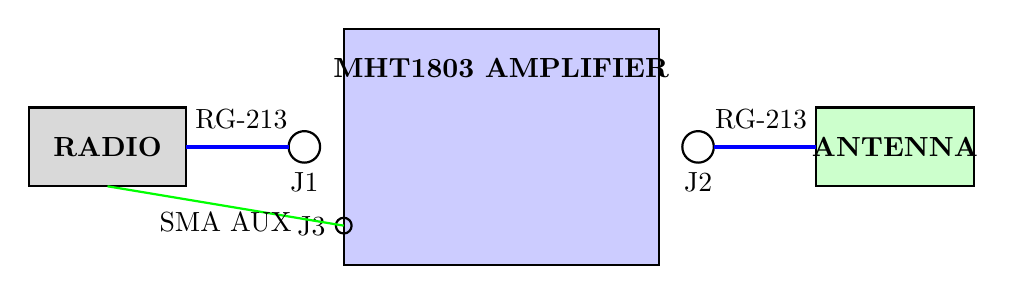
\begin{tikzpicture}[thick]
% Radio
\draw[fill=gray!30] (0,1) rectangle (2,2);
\node at (1,1.5) {\textbf{RADIO}};

% Amplifier
\draw[fill=blue!20] (4,0) rectangle (8,3);
\node at (6,2.5) {\textbf{MHT1803 AMPLIFIER}};

% Antenna
\draw[fill=green!20] (10,1) rectangle (12,2);
\node at (11,1.5) {\textbf{ANTENNA}};

% Connectors
\draw (3.5,1.5) circle (0.2);
\node[below] at (3.5,1.3) {J1};
\draw (8.5,1.5) circle (0.2);
\node[below] at (8.5,1.3) {J2};
\draw (4,0.5) circle (0.1);
\node[left] at (3.9,0.5) {J3};

% RF paths
\draw[blue,very thick] (2,1.5) -- (3.3,1.5);
\draw[blue,very thick] (8.7,1.5) -- (10,1.5);
\draw[green,thick] (1,1) -- (4,0.5);

% Labels
\node[above] at (2.7,1.6) {RG-213};
\node[above] at (9.3,1.6) {RG-213};
\node[below] at (2.5,0.8) {SMA AUX};
\end{tikzpicture}
\end{center}

\textbf{RF Connection Procedure:}
\begin{enumerate}
    \item Connect radio output to J1 (SO-239 Input) using RG-213 coax
    \item Connect J2 (SO-239 Output) to antenna system using RG-213 coax
    \item Optional: Connect auxiliary radio to J3 (SMA connector)
    \item Verify all connections are tight and weatherproofed
    \item Check SWR with antenna analyzer before operation
\end{enumerate}

\section{Operation}

\subsection{Control Panel Layout}

\begin{center}
\begin{tikzpicture}[scale=0.8]
% Panel outline
\draw[thick] (0,0) rectangle (12,4);
\node[above] at (6,4.2) {\textbf{Front Panel Controls}};

% Band selector
\draw (2,2) circle (0.8);
\draw (2,2) circle (0.6);
\node at (2,0.8) {\textbf{BAND SELECT}};
\node[tiny] at (2,3.2) {10M};
\node[tiny] at (3,2.6) {12M};
\node[tiny] at (3,1.4) {20M};
\node[tiny] at (1,1.4) {40M};
\node[tiny] at (1,2.6) {80M};

% Mode selector  
\draw (5,1.5) rectangle (7,2.5);
\node at (6,0.8) {\textbf{MODE SELECT}};
\node[tiny] at (5.3,2) {AM};
\node[tiny] at (6,2) {SSB};
\node[tiny] at (6.7,2) {FM};

% LEDs
\draw[fill=green] (9,3) circle (0.2);
\node[below] at (9,2.7) {POWER};
\draw[fill=red] (10.5,3) circle (0.2);
\node[below] at (10.5,2.7) {OVERHEAT};

% Labels
\node at (9.75,1) {\textbf{STATUS INDICATORS}};
\end{tikzpicture}
\end{center}

\subsection{Pre-Operation Checklist}
\begin{enumerate}
    \item Verify AIO cooler is operating (fan spinning, coolant flowing)
    \item Check power connections are secure
    \item Confirm antenna SWR is acceptable (<2:1)
    \item Set band selector to operating band
    \item Set mode selector to desired mode (AM/SSB/FM)
    \item Verify radio is set to low power (6-8W output)
\end{enumerate}

\subsection{Power-Up Sequence}
\begin{enumerate}
    \item Turn on AIO cooler system first
    \item Wait 30 seconds for coolant circulation
    \item Switch on main power (Power LED should illuminate green)
    \item Allow 2-minute warm-up period
    \item Check that Overheat LED remains off
    \item Amplifier is ready for operation
\end{enumerate}

\subsection{Operating Procedure}

\subsubsection{Band Selection}
Rotate the 5-position band selector switch to match your operating frequency:
\begin{itemize}
    \item \textbf{Position 1:} 80 meters (3.5-4.0 MHz)
    \item \textbf{Position 2:} 40 meters (7.0-7.3 MHz)  
    \item \textbf{Position 3:} 20 meters (14.0-14.35 MHz)
    \item \textbf{Position 4:} 12 meters (24.89-24.99 MHz)
    \item \textbf{Position 5:} 10 meters (28.0-29.7 MHz)
\end{itemize}

\subsubsection{Mode Selection}
Set the 3-position mode switch according to your transmission mode:
\begin{itemize}
    \item \textbf{AM:} Amplitude Modulation (carrier + sidebands)
    \item \textbf{SSB:} Single Sideband (USB/LSB)
    \item \textbf{FM:} Frequency Modulation (repeater operation)
\end{itemize}

\subsubsection{Transmission}
\begin{enumerate}
    \item Verify band and mode settings are correct
    \item Ensure radio output power is set to 6-8 watts
    \item Key the radio briefly (1-2 seconds) to verify operation
    \item Monitor Power LED (should remain green)
    \item Monitor Overheat LED (should remain off)
    \item Proceed with normal operation
\end{enumerate}

\subsection{LED Status Indicators}

\begin{center}
\begin{tabular}{|l|l|l|}
\hline
\textbf{LED} & \textbf{Status} & \textbf{Meaning} \\
\hline
Power (Green) & ON & Normal operation, DC power OK \\
Power (Green) & OFF & No DC power or fuse blown \\
Power (Green) & Blinking & DC voltage low (<11V) \\
\hline
Overheat (Red) & OFF & Temperature normal (<85°C) \\
Overheat (Red) & ON & Overtemperature protection active \\
Overheat (Red) & Blinking & Thermal sensor fault \\
\hline
\end{tabular}
\end{center}

\section{Troubleshooting}

\subsection{No Power (Power LED Off)}
\textbf{Possible Causes and Solutions:}
\begin{itemize}
    \item \textbf{Blown fuse:} Check and replace 30A fuse
    \item \textbf{Loose connections:} Verify all power connections are tight
    \item \textbf{Low battery voltage:} Check battery voltage (should be >11V)
    \item \textbf{Faulty power switch:} Test switch continuity
\end{itemize}

\subsection{Overheat LED On}
\textbf{Immediate Actions:}
\begin{enumerate}
    \item Stop transmitting immediately
    \item Verify AIO cooler operation
    \item Allow amplifier to cool for 10 minutes
    \item Check for blocked airflow
\end{enumerate}

\textbf{Possible Causes:}
\begin{itemize}
    \item AIO cooler pump failure
    \item Radiator airflow blockage
    \item High ambient temperature
    \item Excessive duty cycle
    \item Thermal paste degradation
\end{itemize}

\subsection{No RF Output}
\textbf{Check the following:}
\begin{itemize}
    \item Input drive level (should be 6-8W)
    \item Band selector position
    \item Antenna SWR (<2:1)
    \item RF connections are secure
    \item Mode selector setting matches radio
\end{itemize}

\subsection{Reduced Power Output}
\textbf{Possible Causes:}
\begin{itemize}
    \item Low input drive power
    \item High SWR
    \item Thermal limiting
    \item Low supply voltage
    \item Component aging
\end{itemize}

\subsection{Error Codes and Diagnostics}

\begin{center}
\begin{tabular}{|l|l|l|}
\hline
\textbf{LED Pattern} & \textbf{Code} & \textbf{Problem} \\
\hline
Power: 1 blink, pause & E01 & Input undervoltage \\
Power: 2 blinks, pause & E02 & Output overvoltage \\
Power: 3 blinks, pause & E03 & VSWR protection \\
Overheat: Fast blink & E04 & Thermal sensor fault \\
Both LEDs alternating & E05 & System fault \\
\hline
\end{tabular}
\end{center}

\section{Maintenance}

\subsection{Routine Maintenance Schedule}

\subsubsection{Monthly Checks}
\begin{itemize}
    \item Verify AIO cooler operation
    \item Check power connections for tightness
    \item Clean external surfaces
    \item Inspect RF connectors for corrosion
\end{itemize}

\subsubsection{Quarterly Maintenance}
\begin{itemize}
    \item Check coolant level (if serviceable)
    \item Inspect mounting hardware
    \item Verify grounding connections
    \item Test protection circuits
\end{itemize}

\subsubsection{Annual Service}
\begin{itemize}
    \item Replace thermal paste on MOSFETs
    \item Comprehensive electrical testing
    \item AIO cooler system service
    \item Calibration verification
\end{itemize}

\subsection{Cleaning Procedures}
\begin{enumerate}
    \item Disconnect all power before cleaning
    \item Use only isopropyl alcohol and lint-free cloths
    \item Avoid getting moisture in connectors or controls
    \item Allow to dry completely before reconnecting power
\end{enumerate}

\subsection{Storage Recommendations}
\begin{itemize}
    \item Store in dry, temperature-controlled environment
    \item Protect connectors with caps
    \item Drain AIO cooler if storing below freezing
    \item Check condition every 6 months during storage
\end{itemize}

\section{Technical Specifications}

\subsection{RF Performance}
\begin{center}
\begin{tabular}{|l|l|}
\hline
\textbf{Parameter} & \textbf{Specification} \\
\hline
Frequency Range & 1.8 - 30 MHz \\
Power Output & 500W continuous \\
Input Power & 6 - 8W \\
Gain & 18 - 19 dB \\
Efficiency & >65\% \\
Harmonics & <-40 dBc \\
Spurious & <-50 dBc \\
Input VSWR & <1.5:1 \\
Output VSWR Tolerance & 3:1 maximum \\
\hline
\end{tabular}
\end{center}

\subsection{Electrical Specifications}
\begin{center}
\begin{tabular}{|l|l|}
\hline
\textbf{Parameter} & \textbf{Specification} \\
\hline
Supply Voltage & 12 - 14V DC \\
Current Consumption (Idle) & 2.5A \\
Current Consumption (Full Power) & 45A \\
Internal Voltage & 50V DC \\
Power Consumption & 630W maximum \\
\hline
\end{tabular}
\end{center}

\subsection{Physical Specifications}
\begin{center}
\begin{tabular}{|l|l|}
\hline
\textbf{Parameter} & \textbf{Specification} \\
\hline
Dimensions (W×H×D) & 220 × 80 × 180 mm \\
Weight & 3.2 kg \\
Operating Temperature & -10°C to +50°C \\
Storage Temperature & -40°C to +70°C \\
Humidity & 0-95\% non-condensing \\
Cooling & 240mm AIO liquid cooling \\
\hline
\end{tabular}
\end{center}

\subsection{Connectors and Controls}
\begin{center}
\begin{tabular}{|l|l|l|}
\hline
\textbf{Connector} & \textbf{Type} & \textbf{Function} \\
\hline
J1 & SO-239 & RF Input (from radio) \\
J2 & SO-239 & RF Output (to antenna) \\
J3 & SMA & Auxiliary RF Input \\
J4 & Screw Terminal & 12V DC Power Input \\
SW1 & Rotary (1P5T) & Band Selection \\
SW2 & Slide (1P3T) & Mode Selection \\
D1 & LED (Green) & Power Indicator \\
D2 & LED (Red) & Overheat Indicator \\
\hline
\end{tabular}
\end{center}

\section{Warranty and Support}

\subsection{Warranty Terms}
This amplifier is warranted for a period of two (2) years from date of purchase against defects in materials and workmanship under normal amateur radio use.

\subsection{Warranty Exclusions}
\begin{itemize}
    \item Damage from overvoltage or reverse polarity
    \item Damage from excessive SWR or no-load operation
    \item Damage from modification or improper repair
    \item Normal wear items (thermal paste, coolant)
    \item Damage from environmental factors
\end{itemize}

\subsection{Technical Support}
For technical support, please contact:
\begin{itemize}
    \item Email: support@rfdesign.com
    \item Phone: +1-555-RF-POWER
    \item Web: www.rfdesign.com/support
    \item Hours: Monday-Friday, 8 AM - 5 PM EST
\end{itemize}

\subsection{Service Information}
For service requirements:
\begin{enumerate}
    \item Contact technical support for return authorization
    \item Package unit securely with all accessories
    \item Include detailed description of problem
    \item Allow 2-3 weeks for repair turnaround
\end{enumerate}

\section{Appendices}

\subsection{Appendix A: Band Plan Reference}
\begin{center}
\small
\begin{tabular}{|l|l|l|l|}
\hline
\textbf{Band} & \textbf{Frequency} & \textbf{Wavelength} & \textbf{Typical Use} \\
\hline
80 meters & 3.5 - 4.0 MHz & 80m & Regional/DX \\
40 meters & 7.0 - 7.3 MHz & 40m & Regional/DX \\
20 meters & 14.0 - 14.35 MHz & 20m & Worldwide DX \\
12 meters & 24.89 - 24.99 MHz & 12m & Sporadic E \\
10 meters & 28.0 - 29.7 MHz & 10m & Skip/Local \\
\hline
\end{tabular}
\end{center}

\subsection{Appendix B: SWR Chart}
\begin{center}
\begin{tikzpicture}[scale=0.8]
\draw[->] (0,0) -- (8,0) node[right] {SWR};
\draw[->] (0,0) -- (0,5) node[above] {Power};
\draw[thick,green] (0,4) -- (1.5,4) -- (2,3.8) -- (3,3) -- (4,2) -- (5,1) -- (6,0.5);
\draw[dashed] (2,0) -- (2,5) node[above] {2:1};
\draw[dashed] (3,0) -- (3,5) node[above] {3:1};
\node[below] at (1,0) {1:1};
\node[below] at (4,0) {4:1};
\node[below] at (6,0) {6:1};
\node[left] at (0,4) {100\%};
\node[left] at (0,2) {50\%};
\node[left] at (0,1) {25\%};
\end{tikzpicture}
\end{center}

\subsection{Appendix C: Parts List for User Serviceable Items}
\begin{center}
\begin{tabular}{|l|l|l|}
\hline
\textbf{Item} & \textbf{Part Number} & \textbf{Description} \\
\hline
F1 & LF-30A-32V & 30A Automotive Fuse \\
TH1 & NTC-10K-B3977 & 10K NTC Thermistor \\
Thermal Paste & MX-4-4G & Arctic MX-4 Thermal Compound \\
Coolant & CL-CLEAR-1L & AIO Coolant (Clear) \\
\hline
\end{tabular}
\end{center}

\section{RF Matching Networks}
\label{sec:rf_matching}

The amplifier includes dedicated RF matching networks for each supported band (80m, 40m, 20m, 12m, and 10m). These networks are designed to provide optimal impedance matching between the RF input and the amplifier stages, ensuring maximum power transfer and efficiency.

\subsection{Matching Network Selection}
The matching networks are automatically selected based on the band selection switch position. Each network is optimized for its specific band and includes:
\begin{itemize}
    \item Input impedance matching for 50Ω to the amplifier input impedance
    \item Output impedance matching for the amplifier output to 50Ω
    \item Band-specific filtering to reduce harmonics
\end{itemize}

\subsection{Tuning and Adjustment}
The matching networks are factory-tuned and should not require adjustment. However, if modification is necessary:
\begin{enumerate}
    \item Ensure the amplifier is powered off and disconnected
    \item Remove the top cover to access the matching networks
    \item Use a network analyzer to measure the input/output impedance
    \item Adjust the matching components as needed
    \item Verify the VSWR is below 1.5:1 across the band
\end{enumerate}

\section{VSWR Protection}
\label{sec:vswr_protection}

The amplifier includes a comprehensive VSWR protection circuit to prevent damage from high reflected power conditions.

\subsection{Protection Features}
The VSWR protection circuit provides:
\begin{itemize}
    \item Real-time monitoring of forward and reflected power
    \item Automatic power reduction when VSWR exceeds 2:1
    \item Complete shutdown if VSWR exceeds 3:1
    \item Visual indication of protection activation
\end{itemize}

\subsection{Protection Circuit Operation}
The protection circuit operates as follows:
\begin{enumerate}
    \item Continuously monitors the RF output
    \item Compares forward and reflected power levels
    \item Activates protection if VSWR threshold is exceeded
    \item Automatically resets when conditions return to normal
\end{enumerate}

\section{EMI Filtering}
\label{sec:emi_filtering}

The amplifier includes comprehensive EMI filtering to ensure compliance with regulatory requirements and prevent interference with other equipment.

\subsection{Filter Components}
The EMI filter circuit consists of:
\begin{itemize}
    \item Input line filter for power supply
    \item RF output filtering
    \item Ferrite bead suppression
    \item Decoupling capacitors
\end{itemize}

\subsection{Filter Maintenance}
To maintain proper EMI filtering:
\begin{enumerate}
    \item Keep all filter components clean and dry
    \item Check for physical damage during regular maintenance
    \item Verify filter effectiveness during annual testing
    \item Replace damaged or degraded components immediately
\end{enumerate}

\vfill
\begin{center}
\textbf{END OF MANUAL}\\
\textit{Document Version 1.0 - June 2025}\\
\textit{© 2025 RF Design Engineering - All Rights Reserved}
\end{center}

\end{document}
